\chapter[Structure of the Code]{Structure of the Code}
\label{chap:structure}
%
%
%
\section{Components of GMI}
%
The modules that make up the GMI assessment model are \cite{Rotman-etal01}:
%
\begin{enumerate}
\item Input meteorological data coming from four major Global Circulation
      Models (from NCAR, GISS, DAO, and GMAO). Data from all these input
      sets include horizontal U and V winds, temperature, and surface
      pressure.
\item Advection algorithm to transport trace species
\item Mass tendencies
\item Numerical schemes for chemistry solutions
\item Chemistry mechanism
\item Heterogeneous processes
\item Photolysis
\item Diagnostics
\item Tropospheric treatment
\item Initial conditions
\item Boundary conditions
\end{enumerate}
%
All the above modules have multiple packages/versions that can be selected through
proper resource file settings.
The GMI model incorporates six chemical mechanisms:
\begin{itemize}
\item aerosol (University of Michigan formulation)
\item micro\_aerosol (University of Michigan formulation)
\item gocart\_aerosol (GOCART formulation)
\item stratosphere
\item troposphere
\item combined stratostophere/troposphere (strat\_trop or combo)
\end{itemize}
%
A summary of the mechanisms appears in Table \ref{tab:mecha}.
%

{\small
\begin{center}
\begin{table}[!h]
\begin{tabular}{|l|c|c|c|} \hline\hline
Mechanism name      & $\#$ species & $\#$ thermal reactions & $\#$ photolytic reactions  \\ \hline\hline
aerosol         & 30  &  8  &  1  \\
micro\_aerosol  & 40  &  8  &  1  \\
gocart\_aerosol & 31  &  8  &  1  \\
stratosphere    & 57  & 122 & 44  \\
troposphere     & 85  & 222 & 49  \\
strat\_trop     & 124 & 320 & 81  \\ \hline\hline
\end{tabular}
\caption{Basic information on the chemical mechanisms.}
\label{tab:mecha}
\end{table}
\end{center}
}

%
\section{Directory Structure of The Code}
%
The top directory of the GMI code is {\em gmi\_gsfc/}
which contains the sub-directories 
%
\begin{itemize}
\item {\em Components/}: Routines for each component
\item {\em Shared/}: Include files and routines shared by all the components
\item {\em Documents/}: General information about the code and how it is to be used
\item {\em Applications/}: Routines for driving the code
\item {\em Config/}: Main makefile files
\end{itemize}
%
In Table \ref{ta:gmi_dir4}, 
we give more details on the structure of each of the above directories.

{\small

\begin{landscape}

\begin{center}
\begin{longtable}{|l|l|} \hline \hline
{\bf Directory Name}                & {\bf Synopsis} \\ \hline\hline
{\bf gmi\_gsfc }                          & GMI reference directory \\ \hline
gmi\_gsfc/Documents                       & Directory for documents                 \\ \hline
gmi\_gsfc/Documents/Papers                &                                       \\ \hline
gmi\_gsfc/Documents/Tutorials             &                         \\ \hline
gmi\_gsfc/Documents/Tutorials/UserGuide   & This document           \\ \hline
gmi\_gsfc/Documents/Tutorials/removingESM   &                         \\ \hline
gmi\_gsfc/Documents/Tutorials/MEGANemissions &                         \\ \hline
gmi\_gsfc/Documents/ReadmeFiles           &                                       \\ \hline
gmi\_gsfc/Config                          &  Main makefile files \\  \hline
gmi\_gsfc/Shared               & Files and modules shared by all the components \\ \hline
gmi\_gsfc/Shared/GmiCommunications        &  Communication routines             \\ \hline
gmi\_gsfc/Shared/GmiIOutilities         &   Supporting routines for I/O          \\ \hline
gmi\_gsfc/Shared/GmiESMF                &  Interfaces to ESMF                      \\ \hline
gmi\_gsfc/Shared/GmiInclude         &   Include files                              \\ \hline
gmi\_gsfc/Shared/GmiMetFields         &  Routines for deriving MetFields variables   \\ \hline
gmi\_gsfc/Shared/GmiScripts         &   Script tools                                   \\ \hline
gmi\_gsfc/Shared/GmiSupportingModules & Supporting routines for various calculations.  \\ \hline
gmi\_gsfc/Shared/NcUtils\_Double         & netCDF utility routines for double precision \\ \hline
gmi\_gsfc/Shared/NcUtils\_Single         & netCDF utility routines for single precision  \\ \hline
gmi\_gsfc/Components/GmiAdvection        & Advection component \\ \hline
gmi\_gsfc/Components/GmiAdvection/advectionMethod & Routines driving Advection \\ \hline
gmi\_gsfc/Components/GmiAdvection/dao2advec       & DAO advection routines \\ \hline
gmi\_gsfc/Components/GmiAdvection/dao2utils       & Advection utility routine computing, \\
                                             & courant numbers, Divergence, etc. \\ \hline
gmi\_gsfc/Components/GmiAdvection/include     & Advection include file \\ \hline
gmi\_gsfc/Components/GmiChemistry             & Chemistry component  \\ \hline
gmi\_gsfc/Components/GmiChemistry/chemistryMethod  & Routines driving Chemistry \\ \hline
gmi\_gsfc/Components/GmiChemistry/AerosolDust  &  Module for Aerosol/Dust calculations \\ \hline
gmi\_gsfc/Components/GmiChemistry/ioChemistry  &  I/O routines for Chemistry \\ \hline
gmi\_gsfc/Components/GmiChemistry/include     & Chemistry include file \\ \hline
gmi\_gsfc/Components/GmiChemistry/sad  & Aerosol surface area density and condensed   \\
                                             & phase mixing ratio modules \\ \hline
gmi\_gsfc/Components/GmiChemistry/solvers  &  Chemistry solvers \\ \hline
gmi\_gsfc/Components/GmiChemistry/solvers/micro\_sulfur  &  \\ \hline
gmi\_gsfc/Components/GmiChemistry/solvers/smv2chem  &  \\ \hline
gmi\_gsfc/Components/GmiChemistry/solvers/sulfur  &  \\ \hline
gmi\_gsfc/Components/GmiChemistry/mechanisms    & Chemical mechanisms \\ \hline
gmi\_gsfc/Components/GmiChemistry/mechanisms/aerosol                     & Aerosol chemistry \\ \hline
gmi\_gsfc/Components/GmiChemistry/mechanisms/aerosol/include\_setkin     & Include files for aerosol \\ \hline
gmi\_gsfc/Components/GmiChemistry/mechanisms/aerosol/setkin              & Routines for rate constants and kinetic rates \\ \hline
gmi\_gsfc/Components/GmiChemistry/mechanisms/micro\_aerosol  & micro\_aerosol chemistry \\ \hline
gmi\_gsfc/Components/GmiChemistry/mechanisms/micro\_aerosol/include\_setkin     & Include files for micro\_aerosol \\ \hline
gmi\_gsfc/Components/GmiChemistry/mechanisms/micro\_aerosol/setkin              & Routines for rate constants and kinetic rates \\ \hline
gmi\_gsfc/Components/GmiChemistry/mechanisms/gocart\_aerosol & gocart\_aerosol chemistry \\ \hline
gmi\_gsfc/Components/GmiChemistry/mechanisms/gocart\_aerosol/include\_setkin & Include files for gocart\_aerosol \\ \hline
gmi\_gsfc/Components/GmiChemistry/mechanisms/gocart\_aerosol/setkin          & Routines for rate constants and kinetic rates \\ \hline
gmi\_gsfc/Components/GmiChemistry/mechanisms/strat\_trop                 & Strat/Trop chemistry \\ \hline
gmi\_gsfc/Components/GmiChemistry/mechanisms/strat\_trop/include\_setkin & Include files for the combined strat/trop \\ \hline
gmi\_gsfc/Components/GmiChemistry/mechanisms/strat\_trop/setkin          & Routines for rate constants and kinetic rates \\ \hline
gmi\_gsfc/Components/GmiChemistry/mechanisms/stratosphere                & Stratospheric chemistry \\ \hline
gmi\_gsfc/Components/GmiChemistry/mechanisms/stratosphere/include\_setkin& Include files for stratosphere \\ \hline
gmi\_gsfc/Components/GmiChemistry/mechanisms/stratosphere/setkin         & Routines for rate constants and kinetic rates \\ \hline
gmi\_gsfc/Components/GmiChemistry/sulfur                      & Routines for sulfur chemistry \\ \hline
gmi\_gsfc/Components/GmiChemistry/mechanisms/troposphere      & Tropospheric chemistry \\ \hline
gmi\_gsfc/Components/GmiChemistry/mechanisms/troposphere/include\_setkin & Include files for troposphere \\ \hline
gmi\_gsfc/Components/GmiChemistry/mechanisms/troposphere/setkin          & Routines for rate constants and kinetic rates \\ \hline
gmi\_gsfc/Components/GmiChemistry/photolysis & Photolysis component \\ \hline
gmi\_gsfc/Components/GmiChemistry/photolysis/include & \\ \hline
gmi\_gsfc/Components/GmiChemistry/photolysis/fastj & \\ \hline
gmi\_gsfc/Components/GmiChemistry/photolysis/fast\_JX & \\ \hline
gmi\_gsfc/Components/GmiChemistry/photolysis/fast\_JX53b & \\ \hline
gmi\_gsfc/Components/GmiChemistry/photolysis/fast\_JX53c\_ref & \\ \hline
gmi\_gsfc/Components/GmiChemistry/photolysis/lookup & Routines for lookup table \\ \hline
gmi\_gsfc/Components/GmiChemistry/photolysis/utils & \\ \hline
gmi\_gsfc/Components/GmiConvection & Convection component \\ \hline
gmi\_gsfc/Components/GmiConvection/convectionMethod & Routines driving Convection \\ \hline
gmi\_gsfc/Components/GmiDeposition & Deposition component \\ \hline
gmi\_gsfc/Components/GmiDeposition/depositionMethod &  Routines driving Deposition  \\ \hline
gmi\_gsfc/Components/GmiDeposition/include &                     \\ \hline
gmi\_gsfc/Components/GmiDiffusion         & Diffusion component \\ \hline
gmi\_gsfc/Components/GmiDiffusion/diffusionMethod  & Routines driving Diffusion \\ \hline
 gmi\_gsfc/Components/GmiEmission  & Emission component \\ \hline
gmi\_gsfc/Components/GmiEmission/emissionMethod  & Routines driving Emission \\ \hline
gmi\_gsfc/Components/GmiEmission/Harvard & Harvard emission routines \\ \hline
gmi\_gsfc/Components/GmiEmission/MEGAN & MEGAN emission routines \\ \hline
gmi\_gsfc/Components/GmiEmission/ioEmission & I/O routines for Emission \\  \hline
gmi\_gsfc/Components/GmiEmission/include &  \\ \hline
gmi\_gsfc/Components/GmiEmission/lightning & Routines for lightning parameterization  \\ \hline
gmi\_gsfc/Components/GmiEmission/llnl & LLNL emission routines \\ \hline
gmi\_gsfc/Components/GmiSpeciesConcentration & Species Concentration component \\ \hline
gmi\_gsfc/Components/GmiSpeciesConcentration/spcConcentrationMethod & Routines driving Species Concentration\\ \hline
gmi\_gsfc/Components/GmiSpeciesConcentration/ioSpcConcentration & I/O routines for Species Concentration \\ \hline
gmi\_gsfc/Applications & Control and time stepping routines \\ \hline
gmi\_gsfc/Applications/GmiApp &  \\ \hline
gmi\_gsfc/Applications/GmiBin &  \\ \hline\hline
\caption{GMI code directories}
\label{ta:gmi_dir4}
\end{longtable}
\end{center}

\end{landscape}

}

\section{Coding Principles}
%
A ".F90" (Fortran code) suffix denotes source code files.
The "F90" suffix indicates that the Fortran source contains
preprocessing directives.
Files named with a ".h" suffix are header files that contain
preprocessing directives, variable declarations, parameter definitions,
and common block definitions.
Contents of selected header files are included via $\# include$ statements
at the beginning portion of each of the ".F90" and ".c" files.

To enable multiyear chemistry simulations, the GMI core model was
parallelized to make use of the most powerful computational
platforms available.
The parallel strategy uses a two-dimensional longitude/latitude
domain decomposition whereby each subdomain consists of a number
of contiguous columns having a full vertical extent.
Processors are assigned to subdomains, and variables local to a given
subdomain are stored on the memory of the assigned processor.
Data are transmitted between computational processes, when needed,
in the form of messages.
The number of meshpoints per subdomain may not be uniform, under the
constraint that the decomposition be logically rectangular.
The choice to decompose in only two dimensions is based on the
fact that chemistry, photolysis, and cold sulfate algorithms make
up the vast majority of the computational requirements and are
all either local or column calculations.
These computations require no communication with neighboring grid
zones and hence maximize the parallel efficiency
\cite{Rotman-etal01}.
 
\section{General Flowchart of the Code}
%
In this section, we provide flowcharts of the main program and the time stepping
routine. 
The main program is {\em gmiMain} (filename gmiMain.F90).
This calls routines to initialize the ESMF programming environment
(that launches the Message Passing Interface MPI),  perform domain decomposition, 
initialize the GMI
components (Chemistry, Emission, Deposition, Advection, Convection, and Diffusion),
perfom model integration (run the components), and finalize the components
and ESMF (see Figure \ref{fig:main}).
%
%
%
\begin{figure}[hbtp]
\centering                                             % center the figure
\includegraphics[height=6.0in,width=6.0in]{gmiMainFlowchart.ps}
\caption{Flowchart of the main program} 
\label{fig:main}
\end{figure}
%
The most important calculations done in the time stepping routine appear in
Figure \ref{fig:step}.
The figure only shows the main modules of the code.
We observe that the major components are executed here.
%
\begin{figure}[hbtp]
\centering                                             % center the figure
\includegraphics[height=7.95in,width=6.50in]{gmiSteppingFlowchart.ps}
\caption{Flowchart of the time stepping routine.}
\label{fig:step}
\end{figure}

